\documentclass[margin,line,11pt]{resume}
 
% \usepackage[latin1]{inputenc}
\usepackage[english,french]{babel}
\usepackage[T1]{fontenc}
\usepackage{fontawesome}
\usepackage{graphicx,wrapfig}
\usepackage{url}
\usepackage[colorlinks=true, pdfstartview=FitV, linkcolor=blue, citecolor=blue, urlcolor=blue]{hyperref}
% \pdfcompresslevel=9

\usepackage[UTF8]{ctex}
\begin{document}{\sc \Huge 孟强}

\begin{resume}

% === PICTURE ===

    % \vspace{0.5cm}
    % \begin{wrapfigure}{R}{0.15\textwidth}
    %      \vspace{-0.9cm}
    %     \begin{center}
    %     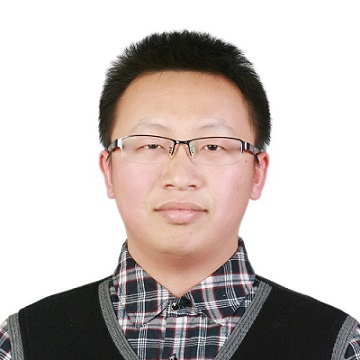
\includegraphics[width=0.11\textwidth]{face}
    %     \end{center}
    %      \vspace{-1cm}
    % \end{wrapfigure}

% === PERSONAL INFO ===
 
            \vspace{-0.5em}\section{\mysidestyle 联系方式}
    \textbf{邮箱}:\hspace{1.5em}  IrvingMeng@outlook.com \\
    \textbf{电话}: \hspace{1.5em} (206)-409-4201\\ 
    \textbf{地址}: \hspace{1.5em}9522 1st Ave NE Apt B6\\
     \hspace*{4.5em}Seattle, WA, 98115 

%             \vspace{-0.5em}\section{\mysidestyle  Objective}
%  To obtain a full-time position in the field of machine learning and data science, applying my knowledge in machine learning, artificial intelligence, optimization, and programming.

             \vspace{-0.5em}\section{\mysidestyle 教育经历}
     \textbf{University of Washington  \hfill WA, USA}\\
Ph.D. Candidate \quad  Industrial and System Engineering \hfill \textit{Sep 2015 - present}\\
 GPA: 3.7/4.0 \vspace{-1em}

 \textbf{中国科学技术大学 \hfill 安徽合肥}\\
工程硕士 \quad 精密机械与精密仪器系 \hfill \textit{Jun 2015}\\
 GPA: 3.78/4.3 (排名: 3/61)
           
% === OBJECTIVE ===

    %         \vspace{-0.5em}\section{\mysidestyle Professional Objective}
    % Improve the efficiency of the microwave and RF designers and structures. I focus on nonlinear devices at circuits level (such as HEMTs transistors) and at system level (HPA, Switches). That purpose requires an original use of an advanced RF instrumentation associated to a strong knowledge in terms of measured devices modeling.
 
% === SKILLS ===
     

% === AWARDS ===

                \vspace{-0.5em}\section{\mysidestyle 获奖情况}
        \begin{list2}
        \item {Teaching Assistant, University of Washington, 2016-2018}
                \item {College of Engineering Dean's Fellowship, University of Washington, 2015-2016}          
        \item {三星奖学金 ,中国科学技术大学, 2014-2015}
        \item {国家励志奖学金, 中国科学技术大学,  2013-2014}
        \item {大学生创新计划一等奖, 中国科学技术大学, 2013}          
        \item {国家励志奖学金,中国科学技术大学, 2012-2013}          
        \item {机器人大赛冠军, 中国科学技术大学, 2012}
        \end{list2}

                \vspace{-0.5em}\section{\mysidestyle 出版文献}
        Huang, Y., \textbf{Meng, Q.}, Evans, H., Lober, W., Cheng, Y., Qian, X., Liu, J. and Huang, S., 2017. CHI: A contemporaneous health index for degenerative disease monitoring using longitudinal measurements. Journal of biomedical informatics, 73, pp.115-124.

        \vspace{-0.5em}
        
       \textbf{Meng, Q.} and Simge, K. , Use mixed-integer optimization to select features under trace ratio criterion combining redundancy constraints and prior knowledge. [\textbf{In progress}]
        
                \vspace{-0.5em}\section{\mysidestyle 选修研究生课程(部分)}
\vspace{0.5em}
	\begin{tabular}{ll }
          \textbf{机器学习} & Machine Learning; Big Data; Artificial Intelligence; Graphical Model; \\
                           &  Non-parametric Process; Markov Decision Process\\
  \textbf{优化} & Linear, Integer Programming; Convex,  Global Optimization \\
   \textbf{统计}& Statistical Inference; Statistical Computing; Time Series \\
\textbf{质量工程} & Quality Control; Design of Experiments \\
	\end{tabular}

 

%         \vspace{-0.5em}\section{\mysidestyle Selected Projects}
%         \begin{list2}
% \item	3 years' professional experience with analytics in digital advertising and sales/marketing fields.
% \item	Proficient in data ETL, visualization, analyzing and modeling with SQL, Excel/VBA, Tableau, Python and R.
% \item	Experienced in designing and conducting strategic projects to identify opportunities for improvements.
% \end{list2}

                \vspace{-0.5em}\section{\mysidestyle 助教课程}
        \begin{list2}
        \item   Probability and Statistics for Engineers; Spring, Summer 2017, Winter, Spring 2018 
        \item   Linear and Network Programming; Autumn 2016, Autumn 2017
        \item  Fundamentals of Engineering Economy; Winter 2016
        \end{list2}
        
         \vspace{-0.5em}\section{\mysidestyle 专业技能}
\vspace{0.5em}
	\begin{tabular}{ll }
\textbf{编程语言} &Python, Matlab, C++, R, Julia, Caffe\\
\textbf{科学软件}& Labview,  AutoCAD, OpenCV\\
	\textbf{实用工具}& Linux, Emacs, Git, \LaTeX, Hadoop
        \end{tabular}

\clearpage        

        \vspace{-0.5em}\section{\mysidestyle 研究项目}

        \textbf{Feature Selection Combining Redundant Information and Prior Knowledge}
\begin{list2}        
\item 提出一个可以结合冗余信息和先验知识选取特征Mixed-integer模型.
\item 深入探究最优解的结构并提出一系列加速求解的方法。加速效果在big data的情况下更加明显。
\item 证明了在Totally Unimodular的情况下,这个NP-hard的问题是polynomial-solvable。
\item 相比于传统的mahine learning算法, mixed-integer模型有应用范围更广,可扩展性更强等优势。现有的实验结果部分验证了该模型的优越性。\textbf{[In progress]}
\end{list2}

\textbf{Contemporaneous Health Index}
\begin{list2}        
\item Developed a novel formulation for contemporaneous patient risk monitoring. This formula translated multivariate longitudinal measurements into a contemporaneous health index (CHI) that captures patient condition changes over the course of progression. The formulation can work in both supervised and unsupervised manner. 
\item Proposed  algorithms to mitigate the challenges associated with the nonsmooth convex optimization problem. Our algorithms involved dual reformulation and block coordinate descent. Extensive numerical studies were performed on both synthetic datasets and real-world applications on Alzheimer's disease and Surgical Site Infection.
\end{list2}

\textbf{机器学习相关的课程项目}
\vspace{0.5 em}
\begin{list2}
\item \textbf{Sparse Principle Component Analysis (sPCA)}.提出了一个结合alternating maximization (AM) method和convex optimization去解决这个NP-hard问题。相比现有算法,该算法保持了组元的正交性并只有微小的方差损失。
\item \textbf{用 Particle Swarm optimization (PSO)训练神经网络}. 该项目用一种叫PSO的全局优化算法去训练神经网络。相比与主流的基于梯度优化和back-propagation的训练方法,该方法能够在训练数据集上得到更高的精度。
% \item \textbf{Parameter tuning of deep neural network}. Played with the CNN on CIFAR data-set with Caffe. 
\item \textbf{用K kernel nearest-neighbor算法完成Netflix competition}. 比较了kNN, Kernal kNN, weighted kNN等非参算法在Netfix问题上的表现. 参数$k$是通过leave-one-out cross validation寻找. 
\item \textbf{Scaling up K-Means with MapReduce}. 用Hadoop MapReduce实现k-means算法将BBC新闻进行分类。 输入试每则新闻的TF-IDF向量.
\item \textbf{PageRank with MapReduce}.用MapReduce完成大矩阵的乘法并找到转移矩阵的stationary分布,从而解决PageRank问题。
\end{list2}


\textbf{强化学习相关的课程项目}
\vspace{0.5 em}
\begin{list2}        
\item \textbf{Cart-pole 问题}. 用基于policy-based的强化学习算法解决寻找根据当前小车状态去保持车上连接杆平衡的策略。 并且比较了两种policy学习的方法(Monte-Carlo policy gradient 和Actor-Critic policy gradient)在本问题的表现。
\item \textbf{Kalah game(美国播棋)}. 用minimax search with alpha-beta pruning作为基本算法。 通过提出不同的heuristic functions建立不同的AIs去和基础AI下棋并给出最优解。
\end{list2}



\textbf{基于视觉导航的室外越障机器人}
\begin{list2}
\item 担任团队队长和程序员。基于openCV开发了能够从杂乱的背景中检测标志并实时导航的系统。该系统在不同的光照,天气和背景情况都能很好地工作。
\item 参与设计了机械结构。该结构能够精确地抓取目标并完成上下楼梯等动作。
\end{list2}






    	

 	

 	       
\end{resume}   
\end{document}